% Adapted from ne630_problems/lesson_27/statement.tex and HW27_Sol.ipynb,
% commit 9c3dc61. Source-based draft: no current HW27 assignment file found.
% Correct ambiguous insertion/removal wording; use the signed rho histories.
\noindent\textit{Source-based draft: verify against the assigned HW27.}

\medskip
\noindent\textbf{Problem 1 [FNRP 5.2].}
A slightly enriched uranium reactor initially gets all its fission power
from U-235. At end of core life, 30\% comes from bred Pu-239. Calculate
the delayed-neutron fraction at beginning and end of life and its percent change.

\begin{adaptedsolution}
Assume equal energy release per fission and equal neutron importance for
the two species. Fission fractions are then 0.7 and 0.3 at EOC, but delayed
fractions must be weighted by \emph{neutron production}, not directly by power.
With $(\nu_{235},\nu_{239})=(2.43,2.90)$ and
$(\beta_{235},\beta_{239})=(0.0065,0.0021)$,
\[
\boxed{\beta_{BOC}=0.0065},\qquad
\boxed{\beta_{EOC}=
\frac{0.7(2.43)(0.0065)+0.3(2.90)(0.0021)}{0.7(2.43)+0.3(2.90)}
=0.00501109}.
\]
The relative change is
$\boxed{100(\beta_{EOC}/\beta_{BOC}-1)=-22.91\%}$.
This is a production-weighted surrogate for an effective delayed fraction.
A true spatial/energy importance-weighted $\beta_{eff}$ requires an adjoint
or equivalent transport treatment, not just the power fractions.
\end{adaptedsolution}

\newpage
\noindent\textbf{Problem 2.}
An initially critical U-235 reactor has $n_0=10^6~\mathrm{cm^{-3}}$,
equilibrium precursors, and $\Lambda=50\times10^{-6}$ s. Solve the six-group
point-kinetics equations and plot $n(t)$ over $0\le t\le10$ s for
\[
\rho(t)=\begin{cases}
0,&0\le t<1,\\
\rho_s,&1\le t<6,\\
0,&6\le t\le10,
\end{cases}\qquad
\text{(a) }\rho_s=+0.25\beta,\quad\text{(b) }\rho_s=-0.25\beta.
\]
Use the Table 5.1 precursor data. The signed histories above govern:
positive reactivity raises power; insertion of absorber removes reactivity.

\begin{adaptedsolution}
The equations and consistent initial inventories are
\[
\dot n=\frac{\rho-\beta}{\Lambda}n+\sum_{i=1}^6\lambda_i C_i,
\qquad \dot C_i=\frac{\beta_i}{\Lambda}n-\lambda_iC_i,
\qquad C_i(0)=\frac{\beta_i n_0}{\Lambda\lambda_i}.
\]
Here $\beta=\sum_i\beta_i=0.0065$ and $\lambda_i=\ln2/t_{1/2,i}$:
\begin{center}\begin{tabular}{rrrr}
\toprule
$i$&$t_{1/2,i}$ (s)&$\beta_i$&$C_i(0)$ ($\mathrm{cm^{-3}}$)\\\midrule
1&56&0.00021&$3.39322\times10^8$\\
2&23&0.00142&$9.42368\times10^8$\\
3&6.2&0.00128&$2.28985\times10^8$\\
4&2.3&0.00257&$1.70555\times10^8$\\
5&0.61&0.00075&$1.32007\times10^7$\\
6&0.23&0.00027&$1.79183\times10^6$\\\bottomrule
\end{tabular}\end{center}
Restart the integrator exactly at 1 and 6 s. A generic adaptive solver can
otherwise step across or even miss an imposed discontinuity.
\begin{minted}{python}
import numpy as np
from scipy.integrate import solve_ivp
beta_i = np.array([.00021,.00142,.00128,.00257,.00075,.00027])
lam = np.log(2)/np.array([56,23,6.2,2.3,.61,.23])
beta, L, n0 = beta_i.sum(), 50e-6, 1e6
def response(sign):
    y = np.r_[n0, beta_i*n0/(L*lam)]
    pieces = []
    for a,b,rho in [(0,1,0), (1,6,sign*.25*beta), (6,10,0)]:
        def rhs(t,y):
            return np.r_[(rho-beta)*y[0]/L + lam@y[1:],
                         beta_i*y[0]/L - lam*y[1:]]
        s = solve_ivp(rhs, (a,b), y, method="Radau",
                      t_eval=np.linspace(a,b,401),
                      rtol=2e-10, atol=1e-3)
        assert s.success
        pieces.append(s)
        y = s.y[:,-1]
    return pieces
up, down = response(1), response(-1)
\end{minted}
Both $n$ and the precursor inventories are continuous at each switch;
the near-prompt adjustment occurs over a finite short time.
\begin{center}\begin{tabular}{rrrr}
\toprule
$\rho_s/\beta$&$n(1)$&$n(6)$&$n(10)$ ($\mathrm{cm^{-3}}$)\\\midrule
$+0.25$&$1.000000\times10^6$&$1.884542\times10^6$&$1.283494\times10^6$\\
$-0.25$&$1.000000\times10^6$&$6.587321\times10^5$&$8.761338\times10^5$\\\bottomrule
\end{tabular}\end{center}
\begin{figure}[H]\centering
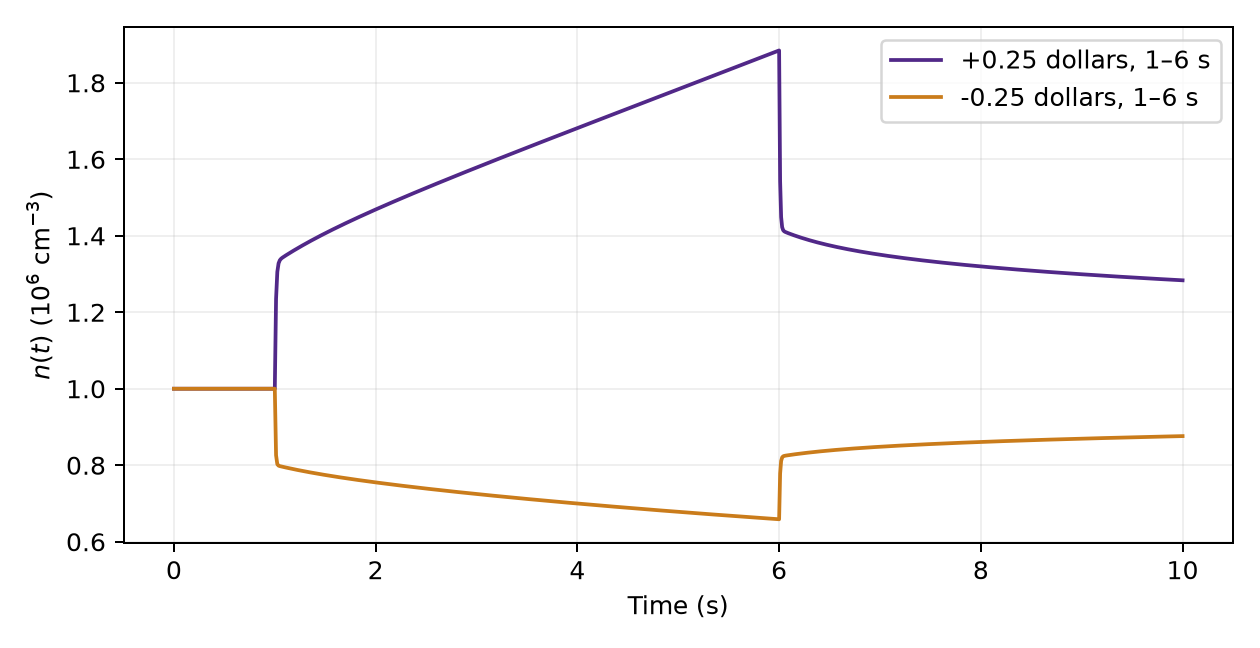
\includegraphics[width=.85\textwidth]{hw27_six_group.png}
\caption{Six-group response to temporary positive and negative reactivity.}
\end{figure}
Returning to zero reactivity does not reset the precursor inventory, so
the final neutron density need not return to its initial value. Each
constant-reactivity interval was checked against the independent matrix
exponential $\mathbf y(b)=e^{A(b-a)}\mathbf y(a)$.
\end{adaptedsolution}
